\documentclass[tikz,border=10pt]{standalone}
\usetikzlibrary{arrows.meta, decorations.markings, calc}

\colorlet{green_set}{green!70!black}
\colorlet{purple_set}{blue!80!cyan!60!red!95!black!90}
\colorlet{red_set}{red!80!black}

% Style for the arrows in the vector field
\tikzset{>=Stealth,
  vector field/.style={
    decoration={markings,
      mark=at position 1 with {\arrow{>[scale=0.6]}}
    },
    postaction={decorate},
    shorten >=0.8pt
  }
}

\begin{document}
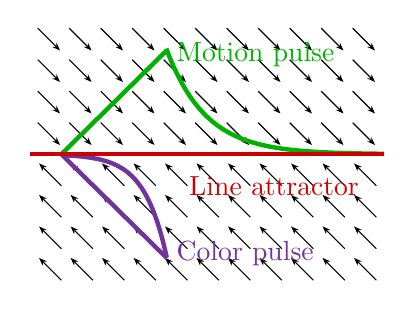
\begin{tikzpicture}[scale=2]

% Draw the vector fields
\foreach \x in {-1,-0.8,...,1}{
  \foreach \y in {-0.8,-0.6,...,-0.2}{
    % Calculate the velocity based on the provided function
    \pgfmathsetmacro{\vx}{0.5*\y}
    \pgfmathsetmacro{\vy}{-0.5*\y}
    % Normalize the velocity for consistent arrow size
    \pgfmathsetmacro{\norm}{sqrt(\vx*\vx+\vy*\vy)}
    \pgfmathsetmacro{\unitvx}{\vx/\norm}
    \pgfmathsetmacro{\unitvy}{\vy/\norm}
    % Draw the vector field arrow
    \draw[vector field] (\x,\y) -- ($(\x,\y)+(\unitvx*0.2,\unitvy*0.2)$);
  }
}

\foreach \x in {-1.15,-0.95,...,1.0}{
  \foreach \y in {0.2,0.4,...,0.8}{
    \pgfmathsetmacro{\vx}{0.5*\y}
    \pgfmathsetmacro{\vy}{-0.5*\y}
    \pgfmathsetmacro{\norm}{sqrt(\vx*\vx+\vy*\vy)}
    \pgfmathsetmacro{\unitvx}{\vx/\norm}
    \pgfmathsetmacro{\unitvy}{\vy/\norm}
    \draw[vector field] (\x,\y) -- ($(\x,\y)+(\unitvx*0.2,\unitvy*0.2)$);
  }
}

% Draw the green line and label it "Motion pulse"
\draw[ultra thick, green_set] (-1,0) -- (-0.33,0.66);
\node[green_set, anchor=south west] at (-0.33,0.49) {Motion pulse};

% Draw the green exponentially decaying curve
\draw[ultra thick, green_set, domain=-0.334:1.05, samples=100] plot (\x, {0.66*exp(-4*(\x + 0.33))});

% Draw the purple line and label it "Color pulse"
\draw[ultra thick, purple_set] (-1,0) -- (-0.33,-0.66);
\node[purple_set, anchor=north west] at (-0.33,-0.49) {Color pulse};

% Draw the purple exponentially decaying curve
\draw[ultra thick, purple_set, domain=-1:-0.33, samples=100] 
  plot (\x, {-0.66 * exp(7*(\x + 0.33))});

% Define the line attractor and label it
\draw[ultra thick, red_set] (-1.2,0) -- (1.05,0);
\node[red_set] at (0.35,-0.2) {Line attractor};

\end{tikzpicture}
\end{document}
